%%%%%%%%%%%%%%%%%%%%%%%%%%%%%%%%%%%%%%%%%%%%%%%%%%%%%%%%%%%%%%%%%%%%%
%                                                                   %
%	CHAPTER TWO, FLECSPH.                                           %
%                                                                   %
%%%%%%%%%%%%%%%%%%%%%%%%%%%%%%%%%%%%%%%%%%%%%%%%%%%%%%%%%%%%%%%%%%%%%
\chapter{Complex simulations on hybrid architectures}

\section{Introduction}

The previous part describes the method we implement to set the last metric of our benchmark for hybrid architectures.
It also presents the wall faced with smoothed particle hydrodynamics and gravitation. 
We showed that this application meets the communication and computation wall in an irregular behavior context. 
We intent to target astrophysical simulation using hybrid architectures. 
This distributed SPH and gravitation implementation is called FleCSPH. 
This is a complex application that, beside of being interesting for our purpose, need to be accurate on the physics aspect to be use by the domain scientists from LANL. 

This section gives details about the FleCSPH framework. 
We first present FleCSI, the base project in the Los Alamos National Laboratory on which FleCSPH is based. 
We then give details on the implementation itself and the tools we implemented to reach a working and efficient code. 
We give details on the domain decomposition strategy used with Morton Ordering. 
The tree traversal algorithm choices are then explained. 

After this presentation of the native code using multi-CPU clusters we present our strategies for a multi-GPU implementation. 
The last section exposes the results for both implementation and the simulations. 

A lot of code already exists for SPH simulation and some are already made using hybrid architectures.
The contribution of FleCSPH is, like FleCSI, to provide a transparent tool for domain scientists. 
Those frameworks provide a bunch of topologies and functions and will handle the load balancing and distribution for the domain scientists. 
This allows the computer scientists to keep track of last hardware evolution and provide efficient algorithms for them while the physicists/astrophysicists/chemists can focus on the simulation itself. 
In this context FleCSPH is focused on tree topologies and will be integrated in FleCSI later on. 

\section{FleCSI}

FleCSI\footnote{\url{http://github.com/laristra/flecsi}}~\cite{bergen2016flexible} is a compile-time configurable framework designed to support multi-physics application development. 
It is developed at the Los Alamos National Laboratory as part of the Los Alamos Ristra project. 
As such, FleCSI provides a very general set of infrastructure design patterns that can be specialized and extended to suit the needs of a broad variety of solver and data requirements. 
FleCSI currently supports multi-dimensional mesh topology, geometry, and adjacency information, as well as n-dimensional hashed-tree data structures, graph partitioning interfaces, and dependency closures.

FleCSI introduces a functional programming model with control, execution, and data abstractions that are consistent both with MPI and with state-of-the-art, task-based runtimes such as Legion\cite{bauer2012legion} and Charm++\cite{kale1993charm++}. 
The abstraction layer insulates developers from the underlying runtime, while allowing support for multiple runtime systems including conventional models like asynchronous MPI.

The intent is to provide developers with a concrete set of user-friendly programming tools that can be used now, while allowing flexibility in choosing runtime implementations and optimization that can be applied to future architectures and runtimes.

FleCSI's control and execution models provide formal nomenclature for describing poorly understood concepts such as kernels and tasks. 
FleCSI's data model provides a low-buy-in approach that makes it an attractive option for many application projects, as developers are not locked into particular layouts or data structure representations.

FleCSI currently provides a parallel but not distributed implementation of Binary, Quad and Oct-tree topology. 
This implementation is based on space filling curves domain decomposition, the Morton order. 
The current version allows the user to specify the code main loop and the data distribution requested. 
The data distribution feature is not available for the tree data structure needed in our SPH code and we provide it in the FleCSPH implementation. 
The next step will be to incorporate it directly from FleCSPH to FleCSI as we reach a decent level of performance.
As FleCSI is an on-development code the structure may change in the future and we keep track of these updates in FleCSPH.

Based on FleCSI the intent is to provide a binary, quad and oct-tree data structure and the methods to create, search and share information for it. 
In FleCSPH this will be dedicated, apply and tested on the SPH method. 
In this part we first present the domain decomposition, based on space filling curves, and the tree data structure.
We describe the HDF5 files structure used for the I/O.
Then we describe the distributed algorithm for the data structure over the MPI processes. 

\section{Distributed SPH on multi-core architecture}
Before going further in the SPH implementation and our development, we need to give details on the algorithm and the work involved. 
%
\begin{algorithm}
\caption{SPH implementation}\label{alg:general_behavior}
\begin{algorithmic}[1]
\State Read particles from file 
\While{not last step}
\State Generate keys for particles 
\State Load balance particles 
\State Generate local tree data structure
\While{Physics not done}
\State Physics: search and distributed search
\State Update data 
\EndWhile
\State Gravitation = FMM
\If{Output step}
\State Output data in H5part format
\EndIf
\EndWhile
\end{algorithmic}
\end{algorithm}
%
The general algorithm is presented on algorithm~\ref{alg:general_behavior} and shows the features of SPH exposed in the previous section. 
In this section we present the main features of our code and the problems involved: the domain decomposition, the tree data structure and traversal and our distribution strategy. 
This project, in collaboration with the LANL, is named FleCSPH. 

FleCSPH\footnote{\url{http://github.com/laristra/flecsph}} is a framework initially created as a part of FleCSI. 
The purpose of FleCSPH is to provide a data distribution and communications patterns to use the tree topology provided in FleCSI applied to SPH.
The final purpose of FleCSPH is to complement the tree topology and provide the \textit{colorer} to FleCSI. 
The distribution strategies associate to a data structure.
As presented in the previous sections, SPH is a very good candidate to benchmark the binary, quad and oct tree topology. 
The demand is high for astrophysics simulation regarding the recent discoveries of the LIGO and the SPH method allows us to generate those simulations. 
\begin{figure}[t!]
\centering
\begin{tikzpicture}
\draw (0,0) rectangle (6,4);
\draw (0,3) rectangle (4,4) node[pos=.5] {\Large \textbf{FleCSI}};
\node [text width=3cm,anchor=north west] at (0.2,2.7) { 
	\textbf{Runtimes:} 
    \begin{itemize}[noitemsep,nolistsep]
        \item[-]{Legion}
        \item[-]{MPI}
        \item[-]{HPX}
        \item[-]{\color{black!40}{Charm++}}
    \end{itemize}
};
\node [text width=2.7cm,anchor=north west] at (3.2,2.7) { 
	\textbf{Topologies:} 
    \begin{itemize}[noitemsep,nolistsep]
        \item[-]{Set}
        \item[-]{Mesh}
        \item[-]{Tree}
        \item[-]{\color{black!40}{Graph}}
    \end{itemize}
};
\node[draw,minimum width=1.7cm,minimum height=.45cm] at (4.7,.95) (tree) {};% rectangle (5.5,1.2) node (tree) {};
\draw (tree.north east) -- (8,4);
\draw (tree.south east) -- (8,0);
\draw (8,0) rectangle (16,4);
\draw (8,3) rectangle (12,4) node[pos=.5] {\Large \textbf{FleCSPH}};
\node [text width=3cm,anchor=north west] at (8.2,2.7) { 
	\textbf{Runtime:} MPI 
	\textbf{Tree:} 
    \begin{itemize}[noitemsep,nolistsep]
        \item[-]{Policy}
        \item[-]{Partitioning}
        \item[-]{Colorer}
    \end{itemize}
};
\node [text width=4cm,anchor=north west] at (11.5,2.7) { 
	\textbf{Physics:} 
    \begin{itemize}[noitemsep,nolistsep]
    	\item[-]{SodTube/Sedov}
    	\item[-]{Fluids}
        \item[-]{Astrophysics}
    \end{itemize}
    \textbf{Plus:} I/O
};
\end{tikzpicture}
\caption{FleCSI and FleCSPH frameworks }
\label{fig:flecsi_flecsph_framework}
\end{figure}
Figure~\ref{fig:flecsi_flecsph_framework} presents how FleCSI and FleCSPH are integrated. 
FleCSPH is based on the tree topology of FleCSI and follows the same structure define in FleCSI. 
The ideal runtime in FleCSI is Legion but this in-development code does not allow us to do more than static data distribution. 
This is why we decided to work with the MPI runtime in FleCSPH. 
Those MPI functions can then be integrated to FleCSI to generate group of particles and labeled them, the coloring. 

\begin{figure}[t!]
\centering
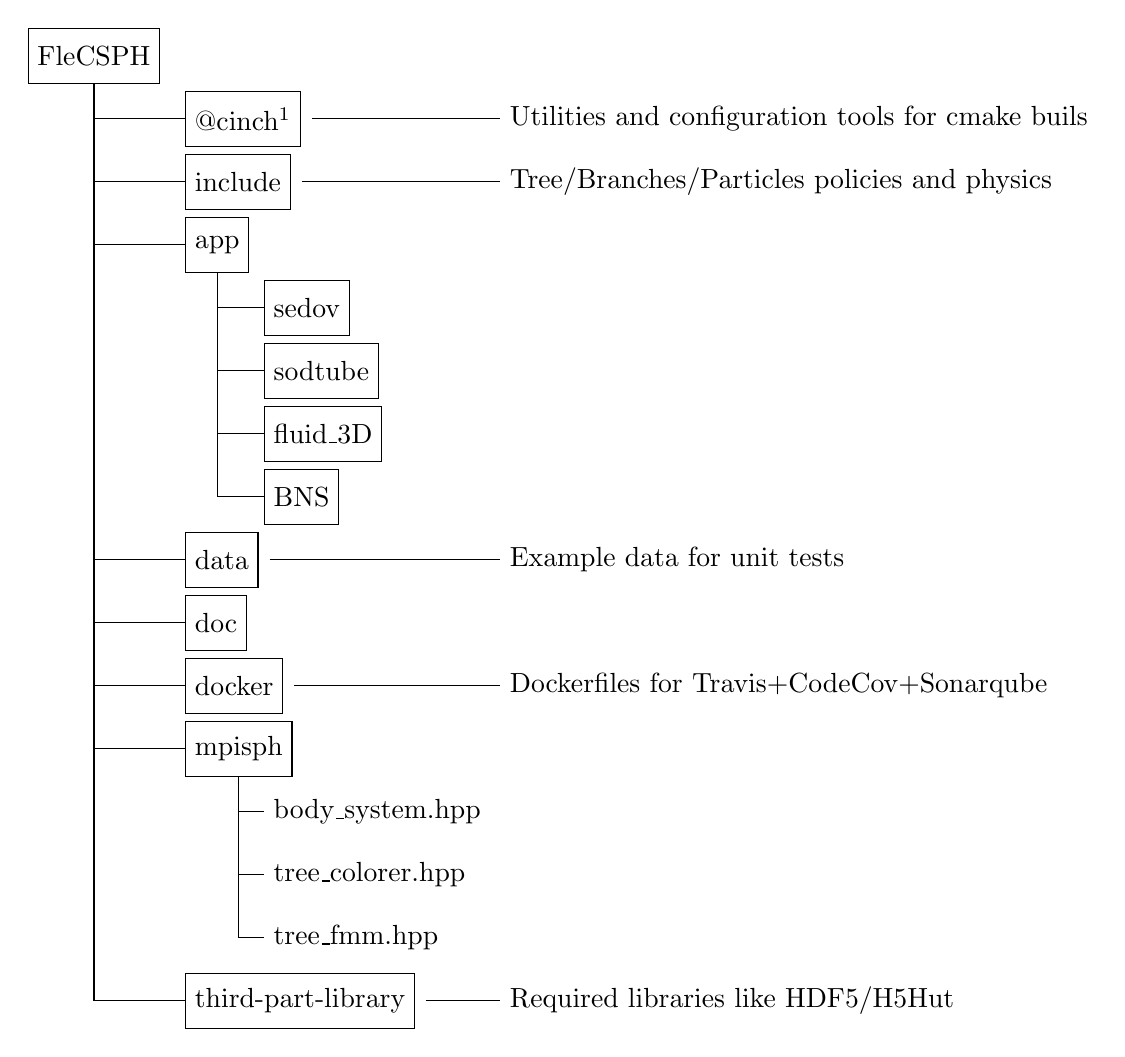
\begin{tikzpicture}
	\def\dist{.8}
	\def\y{10}

	\node[draw,anchor=west,minimum height=.7cm] at (0,\y) (flecsph) {FleCSPH};

	\pgfmathparse{\y-\dist}\edef\y{\pgfmathresult}
	\node[draw,anchor=west,minimum height=.7cm] at (2,\y) (cinch) {@cinch\footnote{https://www.github.com/laristra/cinch}};
	\draw (flecsph.south) |- (cinch.west) -| (cinch.west); 
	\node[anchor=west] at (6,\y) (text) {Utilities and configuration tools for cmake buils};
	\draw ([xshift=4pt]cinch.east) -- ([xshift=-5pt]text);

	\pgfmathparse{\y-\dist}\edef\y{\pgfmathresult}
	\node[draw,anchor=west,minimum height=.7cm] at (2,\y) (include) {include};
	\draw (flecsph.south) |- (include.west) -| (include.west); 
	\node[anchor=west] at (6,\y) (text) {Tree/Branches/Particles policies and physics};
	\draw ([xshift=4pt]include.east) -- ([xshift=-5pt]text);

	\pgfmathparse{\y-\dist}\edef\y{\pgfmathresult}
	\node[draw,anchor=west,minimum height=.7cm] at (2,\y) (app) {app};
	\draw (flecsph.south) |- (app.west) -| (app.west); 
	\pgfmathparse{\y-\dist}\edef\y{\pgfmathresult}
	\node[draw,anchor=west,minimum height=.7cm] at (3,\y) (sedov) {sedov};
	\draw (app.south) |- (sedov.west) -| (sedov.west); 
	\pgfmathparse{\y-\dist}\edef\y{\pgfmathresult}
	\node[draw,anchor=west,minimum height=.7cm] at (3,\y) (sodtube) {sodtube};
	\draw (app.south) |- (sodtube.west) -| (sodtube.west); 
	\pgfmathparse{\y-\dist}\edef\y{\pgfmathresult}
	\node[draw,anchor=west,minimum height=.7cm] at (3,\y) (fluid3D) {fluid\_3D};
	\draw (app.south) |- (fluid3D.west) -| (fluid3D.west); 
	\pgfmathparse{\y-\dist}\edef\y{\pgfmathresult}
	\node[draw,anchor=west,minimum height=.7cm] at (3,\y) (bns) {BNS};
	\draw (app.south) |- (bns.west) -| (bns.west); 

	\pgfmathparse{\y-\dist}\edef\y{\pgfmathresult}
	\node[draw,anchor=west,minimum height=.7cm] at (2,\y) (data) {data};
	\draw (flecsph.south) |- (data.west) -| (data.west);
	\node[anchor=west] at (6,\y) (text) {Example data for unit tests};
	\draw ([xshift=4pt]data.east) -- ([xshift=-5pt]text); 

	\pgfmathparse{\y-\dist}\edef\y{\pgfmathresult}
	\node[draw,anchor=west,minimum height=.7cm] at (2,\y) (doc) {doc};
	\draw (flecsph.south) |- (doc.west) -| (doc.west); 

	\pgfmathparse{\y-\dist}\edef\y{\pgfmathresult}
	\node[draw,anchor=west,minimum height=.7cm] at (2,\y) (docker) {docker};
	\draw (flecsph.south) |- (docker.west) -| (docker.west); 
	\node[anchor=west] at (6,\y) (text) {Dockerfiles for Travis+CodeCov+Sonarqube};
	\draw ([xshift=4pt]docker.east) -- ([xshift=-5pt]text); 

	\pgfmathparse{\y-\dist}\edef\y{\pgfmathresult}
	\node[draw,anchor=west,minimum height=.7cm] at (2,\y) (mpisph) {mpisph};
	\draw (flecsph.south) |- (mpisph.west) -| (mpisph.west); 
	\pgfmathparse{\y-\dist}\edef\y{\pgfmathresult}
	\node[anchor=west,minimum height=.7cm] at (3,\y) (file) {body\_system.hpp};
	\draw (mpisph.south) |- (file.west) -| (file.west); 
	\pgfmathparse{\y-\dist}\edef\y{\pgfmathresult}
	\node[anchor=west,minimum height=.7cm] at (3,\y) (file) {tree\_colorer.hpp};
	\draw (mpisph.south) |- (file.west) -| (file.west); 
	\pgfmathparse{\y-\dist}\edef\y{\pgfmathresult}
	\node[anchor=west,minimum height=.7cm] at (3,\y) (file) {tree\_fmm.hpp};
	\draw (mpisph.south) |- (file.west) -| (file.west); 


	\pgfmathparse{\y-\dist}\edef\y{\pgfmathresult}
	\node[draw,anchor=west,minimum height=.7cm] at (2,\y) (third) {third-part-library};
	\draw (flecsph.south) |- (third.west) -| (third.west); 
	\node[anchor=west] at (6,\y) (text) {Required libraries like HDF5/H5Hut};
	\draw ([xshift=4pt]third.east) -- ([xshift=-5pt]text); 

\end{tikzpicture}
\caption{FleCSPH structures and files}
\label{fig:files_flecsph}
\end{figure}

Figure~\ref{fig:files_flecsph} present the file systems of the github repository. 
We use the tools from Cinch\footnote{\url{http://github.com/laristra/cinch}} developed at LANL for the CMake and the makefile generation. 
It also provides the GoogleTests API for our unit tests. 
The FleCSPH code is currently public and available on github under the \textit{laristra} (Los Alamos Ristra) project.
The continuous integration is ensured by using Travis based on Docker and \textit{Dockerfiles} provided in the Docker folder. 
In addition to Travis for the unit tests we use use tools as CodeCov\footnote{\url{http://codecov.io}} for the code coverage and SonarQube\footnote{\url{http://sonarqube.org/}} for the quality gates. 
In the current version we use external libraries: HDF5, H5hut and a specific library for I/O based on H5hut. 
Those elements are present and installed using scripts in \textit{third-part-library} folder. 

\begin{figure}[t!]
\centering
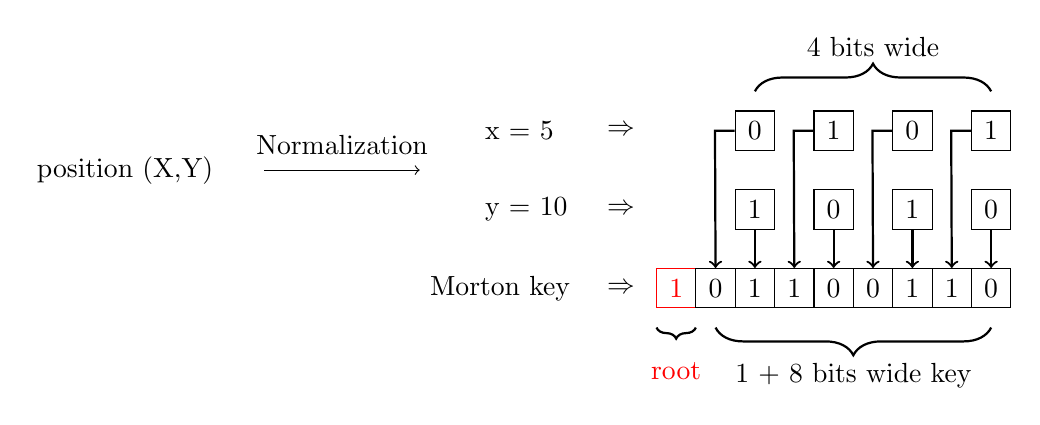
\begin{tikzpicture}

\node at (-6,4.5) (base) {position (X,Y)};
\draw[->] ([xshift=15pt]base.east) -- ([xshift=2.5cm]base.east) node[yshift=2pt,midway,above] () {Normalization};

\node[anchor=west] at (-1.55,5) {x = 5 };
\node[anchor=west] at (-1.55,4) {y = 10 };
\node[anchor=west] at (-2.25,3) {Morton key};

\node[anchor=west] at (0,5) {$\Rightarrow$};
\node[anchor=west] at (0,4) {$\Rightarrow$};
\node[anchor=west] at (0,3) {$\Rightarrow$};

\node[draw,minimum width = .5cm, minimum height = .5cm] at (2,5) (x0) {0};
\node[draw,minimum width = .5cm, minimum height = .5cm] at (3,5) (x1) {1};
\node[draw,minimum width = .5cm, minimum height = .5cm] at (4,5) (x2) {0};
\node[draw,minimum width = .5cm, minimum height = .5cm] at (5,5) (x3) {1};

\node[draw,minimum width = .5cm, minimum height = .5cm] at (2,4) (y0) {1};
\node[draw,minimum width = .5cm, minimum height = .5cm] at (3,4) (y1) {0};
\node[draw,minimum width = .5cm, minimum height = .5cm] at (4,4) (y2) {1};
\node[draw,minimum width = .5cm, minimum height = .5cm] at (5,4) (y3) {0};

% Result
\node[draw,minimum width = .5cm, minimum height = .5cm,red] at (1,3) (root) {1};
%\node[red] at ([yshift=-10pt]root.south) {root};

\node[draw,minimum width = .5cm, minimum height = .5cm] at (1.5,3) (k0) {0};
\node[draw,minimum width = .5cm, minimum height = .5cm] at (2,3) (k1) {1};
\node[draw,minimum width = .5cm, minimum height = .5cm] at (2.5,3) (k2) {1};
\node[draw,minimum width = .5cm, minimum height = .5cm] at (3,3) (k3) {0};
\node[draw,minimum width = .5cm, minimum height = .5cm] at (3.5,3) (k4) {0};
\node[draw,minimum width = .5cm, minimum height = .5cm] at (4,3) (k5) {1};
\node[draw,minimum width = .5cm, minimum height = .5cm] at (4.5,3) (k6) {1};
\node[draw,minimum width = .5cm, minimum height = .5cm] at (5,3) (k7) {0};

\draw [thick,decorate,decoration={brace,amplitude=4pt}]
(1.25,2.5) -- (.75,2.5)  node [red,midway,below,yshift=-9pt] 
{root};

\draw [thick,decorate,decoration={brace,amplitude=10pt}]
(5,2.5) -- (1.5,2.5)  node [midway,below,yshift=-9pt] 
{1 + 8 bits wide key};

\draw [thick,decorate,decoration={brace,amplitude=10pt}]
(2,5.5) -- (5,5.5)  node [midway,above,yshift=9pt] 
{4 bits wide};

% Arrows
\draw[thick,->] (y3.south) -- (k7.north);
\draw[thick,->] (y2.south) -- (k5.north);
\draw[thick,->] (y1.south) -- (k3.north);
\draw[thick,->] (y0.south) -- (k1.north);

\draw[thick,->] (x3.west) -- ([xshift=-.25cm]x3.west) -- (k6.north);
\draw[thick,->] (x2.west) -- ([xshift=-.25cm]x2.west) -- (k4.north);
\draw[thick,->] (x1.west) -- ([xshift=-.25cm]x1.west) -- (k2.north);
\draw[thick,->] (x0.west) -- ([xshift=-.25cm]x0.west) -- (k0.north);
%\draw[thick,->] (y2.west) -- (k5.north);
%\draw[thick,->] (y1.west) -- (k3.north);
%\draw[thick,->] (y0.west) -- (k1.north);
\end{tikzpicture}
\caption{Morton order key generation}
\end{figure}

For the first implementation we present the code without considering accelerators. 
We intent to provide an efficient multi-CPU distributed code. 
The description starts with the domain decomposition strategy which is a basic element for the tree implementation.
We explain the tree data structure for the construction and the search of particles along with the distribution strategy.

\subsection{Domain decomposition}
\label{sec:domain_decomposition}
The number of particles can be high and represent a huge amount of data that does not fit in a single node memory. 
This implies the distribution of the particles over several computational nodes. 
As the particles moves during the simulation the static distribution is not possible and they have to be redistributed at some point in the execution. 
Furthermore, this distribution need to keep local particles in the same computation node to optimize the exchanges and computation itself.

A common approach is to distribute the particles over computational nodes using \textit{space filling curves} like in \cite{warren20132hot,springel2005cosmological,bedorf201424}. 
It intends to assign to each particle a key which is based on its spacial coordinates, then sorting particles based on those keys keeps particles grouped locally.
Many space filling curves exists: Morton, Hilbert, Peano, Moore, Gosper, etc.\

This domain decomposition is used in several layers for our implementation. 
On one hand, to spread the particles over all the MPI processes and provide a decent load balancing regarding the number of particles. 
On the other hand, it is also used locally to store efficiently the particles and provide a $O(N log(N))$ neighbor search complexity, instead of $O(N^2)$, using a tree representation describe in part \ref{sec:trees}. 

Several space filling curves can fit our purposes:
\subsubsection*{The Morton curves} \cite{morton1966computer}, or Z-Order, is the most spread method. 
This method can produce irregular shape domain decomposition like shown in green on figure~\ref{fig:space_filling}. 
The main advantage is to be fast to compute, the key is made by interlacing directly the X, Y and Z bits without rotations. 
\subsubsection*{The Hilbert curves} \cite{sagan2012space} are constructed by interlacing bits but also adding rotation based on the Gray code.
This work is based on the Peano curves and also called Hilber-Peano. 
The construction is more complicated than Morton but allows a better distribution. 

\begin{figure}[t!]
\centering
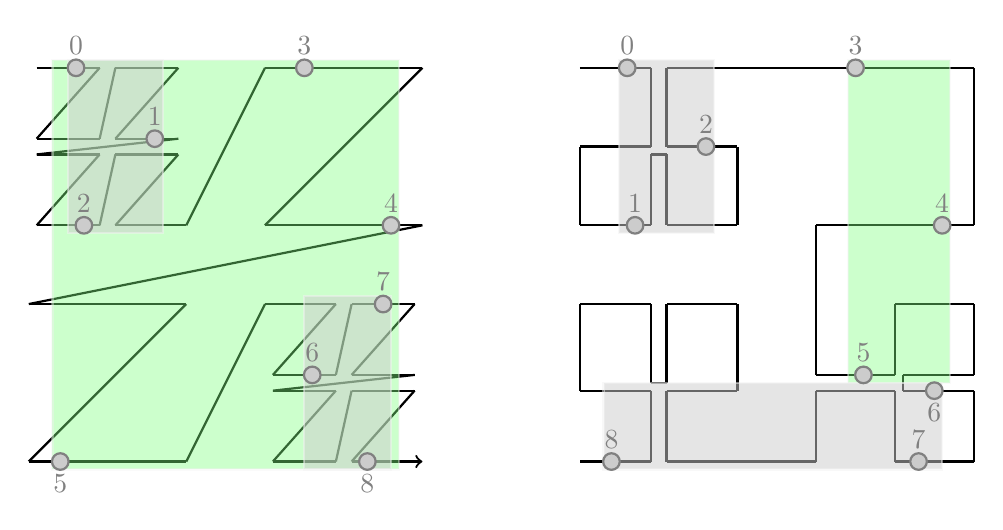
\begin{tikzpicture}[thick]
%\draw[black!50,fill=black!30] (2,2) circle (5pt);
% Morton
\draw[-] (.1,5) -- (.9,5);
\draw[-] (.9,5) -- (.1,4.1);
\draw[-] (.1,4.1) -- (.9,4.1);
\draw[-] (.9,4.1) -- (1.1,5);
\draw[-] (1.1,5) -- (1.9,5);
\draw[-] (1.9,5) -- (1.1,4.1);
\draw[-] (1.1,4.1) -- (1.9,4.1);
\draw[-] (1.9,4.1) -- (0.1,3.9);
\draw[-] (.1,3.9) -- (.9,3.9);
\draw[-] (.9,3.9) -- (.1,3);
\draw[-] (.1,3) -- (.9,3);
\draw[-] (.9,3) -- (1.1,3.9);
\draw[-] (1.1,3.9) -- (1.9,3.9);
\draw[-] (1.9,3.9) -- (1.1,3);
\draw[-] (1.1,3) -- (2,3);

\draw[-] (2,3) -- (3,5);
\draw[-] (3,5) -- (5,5);
\draw[-] (5,5) -- (3,3);
\draw[-] (3,3) -- (5,3);
\draw[-] (5,3) -- (0,2);
\draw[-] (0,2) -- (2,2);
\draw[-] (2,2) -- (0,0);
\draw[-] (0,0) -- (2,0);
\draw[-] (2,0) -- (3,2);

\draw[-] (3,2) -- (3.9,2);
\draw[-] (3.9,2) -- (3.1,1.1);
\draw[-] (3.1,1.1) -- (3.9,1.1);
\draw[-] (3.9,1.1) -- (4.1,2);
\draw[-] (4.1,2) -- (4.9,2);
\draw[-] (4.9,2) -- (4.1,1.1);
\draw[-] (4.1,1.1) -- (4.9,1.1);
\draw[-] (4.9,1.1) -- (3.1,.9);
\draw[-] (3.1,.9) -- (3.9,.9);
\draw[-] (3.9,.9) -- (3.1,0);
\draw[-] (3.1,0) -- (3.9,0);
\draw[-] (3.9,0) -- (4.1,0.9);
\draw[-] (4.1,0.9) -- (4.9,0.9);
\draw[-] (4.9,0.9) -- (4.1,0);
\draw[->] (4.1,0) -- (5,0);

% Hilbert
\draw[-] (7,5) -- (7.9,5);
\draw[-] (7.9,5) -- (7.9,4);
\draw[-] (7.9,4) -- (7,4);
\draw[-] (7,4) -- (7,3);
\draw[-] (7,3) -- (7.9,3);
\draw[-] (7.9,3) -- (7.9,3.9);
\draw[-] (7.9,3.9) -- (8.1,3.9);
\draw[-] (8.1,3.9) -- (8.1,3);
\draw[-] (8.1,3) -- (9,3);
\draw[-] (9,3) -- (9,4);
\draw[-] (9,4) -- (8.1,4);
\draw[-] (8.1,4) -- (8.1,5);
\draw[-] (8.1,5) -- (9,5);

\draw[-] (9,5) -- (10,5);
\draw[-] (10,5) -- (12,5);
\draw[-] (12,5) -- (12,3);
\draw[-] (12,3) -- (10,3);
\draw[-] (10,3) -- (10,2);

\draw[-] (10,2) -- (10,1.1);
\draw[-] (10,1.1) -- (11,1.1);
\draw[-] (11,1.1) -- (11,2);
\draw[-] (11,2) -- (12,2);
\draw[-] (12,2) -- (12,1.1);
\draw[-] (12,1.1) -- (11.1,1.1);
\draw[-] (11.1,1.1) -- (11.1,.9);
\draw[-] (11.1,.9) -- (12,.9);
\draw[-] (12,.9) -- (12,0);
\draw[-] (12,0) -- (11,0);
\draw[-] (11,0) -- (11,.9);
\draw[-] (11,.9) -- (10,.9);
\draw[-] (10,.9) -- (10,0);
\draw[-] (10,0) -- (9,0);

\draw[-] (9,0) -- (8.1,0);
\draw[-] (8.1,0) -- (8.1,.9);
\draw[-] (8.1,.9) -- (9,.9);
\draw[-] (9,.9) -- (9,2);
\draw[-] (9,2) -- (8.1,2);
\draw[-] (8.1,2) -- (8.1,1);
\draw[-] (8.1,1) -- (7.9,1);
\draw[-] (7.9,1) -- (7.9,2);
\draw[-] (7.9,2) -- (7,2);
\draw[-] (7,2) -- (7,.9);
\draw[-] (7,.9) -- (7.9,.9);
\draw[-] (7.9,.9) -- (7.9,0);
\draw[-] (7.9,0) -- (7,0);

% Add the particles over it 
\draw[black!5,opacity=.4,fill=green!50] (.3,-.1) rectangle (4.7,5.1);
\draw[black!5,opacity=0.5,fill=black!20] (.5,2.9) rectangle (1.7,5.1);
\draw[black!5,opacity=0.5,fill=black!20] (3.5,-0.1) rectangle (4.6,2.1);
% P1
\draw[black!50,fill=black!20] (0.6,5) circle (3pt) node[yshift=1pt,above] {0};
\draw[black!50,fill=black!20] (1.6,4.1) circle (3pt) node[yshift=1pt,above] {1};
\draw[black!50,fill=black!20] (.7,3) circle (3pt) node[yshift=1pt,above] {2};
% rect 1 
\draw[black!50,fill=black!20] (3.5,5) circle (3pt) node[yshift=1pt,above] {3};
\draw[black!50,fill=black!20] (4.6,3) circle (3pt) node[yshift=1pt,above] {4};
\draw[black!50,fill=black!20] (.4,0) circle (3pt) node[yshift=-1pt,below] {5};
% rect 1 
\draw[black!50,fill=black!20] (3.6,1.1) circle (3pt) node[yshift=1pt,above] {6};
\draw[black!50,fill=black!20] (4.5,2) circle (3pt) node[yshift=1pt,above] {7};
\draw[black!50,fill=black!20] (4.3,0) circle (3pt) node[yshift=-1pt,below] {8};
% rect 1 


% hilbert rectangles 
\draw[black!5,opacity=.4,fill=green!50] (10.4,1) rectangle (11.7,5.1);
\draw[black!5,opacity=0.5,fill=black!20] (7.5,2.9) rectangle (8.7,5.1);
\draw[black!5,opacity=0.5,fill=black!20] (7.3,-.1) rectangle (11.6,1);

% Hilbert particles
\draw[black!50,fill=black!20] (7.6,5) circle (3pt) node[yshift=1pt,above] {0};
\draw[black!50,fill=black!20] (7.7,3) circle (3pt) node[yshift=1pt,above] {1};
\draw[black!50,fill=black!20] (8.6,4) circle (3pt) node[yshift=1pt,above] {2};

\draw[black!50,fill=black!20] (10.5,5) circle (3pt) node[yshift=1pt,above] {3};
\draw[black!50,fill=black!20] (11.6,3) circle (3pt) node[yshift=1pt,above] {4};
\draw[black!50,fill=black!20] (10.6,1.1) circle (3pt) node[yshift=1pt,above] {5};

\draw[black!50,fill=black!20] (11.5,.9) circle (3pt) node[yshift=-1pt,below] {6};
\draw[black!50,fill=black!20] (11.3,0) circle (3pt) node[yshift=1pt,above] {7};
\draw[black!50,fill=black!20] (7.4,0) circle (3pt) node[yshift=1pt,above] {8};



\end{tikzpicture}
\caption{Morton and Hilbert space filling curves}
\label{fig:space_filling}
\end{figure}

On figure~\ref{fig:space_filling}, the Morton (left) and Hilbert (right) space-filling curves are represented in this example.
The particles are distributed over 3 processes. 
The set of particles of the second process appears in green. 
As we can see there are discontinuities on the Morton case due to the Z-order "jump" over the space. 
This can lead to non-local particles and over-sharing of particles that will not be needed during the computation.
In the Hilbert curve, the locality over the processes is conserved.

In this first implementation of FleCSPH we used the Morton ordering due to the computational cost. 
The next step of this work is to compare the computation time of different space filing curves. 

Technically the keys are generated for each particle at each iteration because their position is expected to change over time. 
To be more efficient, the keys can stay the same during several steps and the final comparison can be made on the real particles positions. 
This increase the search time but allows less tree reconstructions.

We use 64 bits to represent the keys to avoid conflicts.
The FleCSI code allows us to use a combination of memory words to reach the desired size of keys (possibly more than 64 bits) but this will cost in memory occupancy. 
The particle keys are generated by normalizing the space and then converting the floating-point representation to a 64 bits integer for each dimension. 
Then the Morton interlacing is done, and the keys are created. 
Unfortunately, in some arrangements, like isolated particles, or scenarios with very close particles, the keys can be either badly distributed or duplicate keys can appear. 
Indeed, if the distance between two particles is less than $2^{-64} \approx 1$e+$20$, in a normalized space, the key generated through the algorithm will be the same. 
This problem is then handle during the particle sort and then the tree generation. 
In both case two particles can be differentiate based on their unique ID generated at the beginning execution. 

\subsection{Hierarchical trees}
\label{sec:trees}

The method we use for the tree data structure creation and research comes from Barnes-Hut trees presented in \cite{barnes1986hierarchical,barnes1990modified}. 
By reducing the search complexity from $O(N^2)$ for direct summation to $O(Nlog(N))$ it allows us to do very large simulations with billions of particles. 
It also allows the use of the tree data structure to compute gravitation using multipole methods.

We consider binary trees, for 1 dimension, quad-trees, for 2 dimensions, and oct-trees, for 3 dimensions. 
The construction of those trees is directly based on the domain decomposition using keys and space-filling curve presented in section \ref{sec:domain_decomposition}. 

\begin{figure}[t!]
\centering
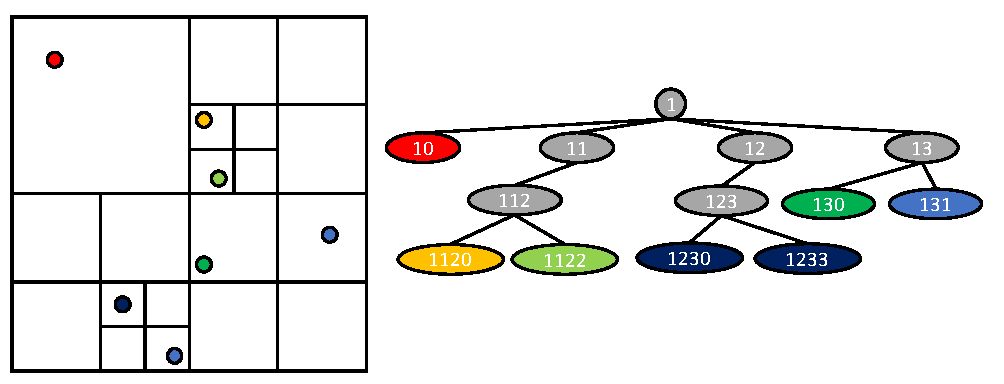
\includegraphics[width=\columnwidth]{\locpath/figures/flecsph/quadtree}
\caption{Quadtree, space and data representation}
\label{fig:quadtree}
\end{figure}

As explain in the previous section, we use 64 bits keys.
That give us up to $63$, $31$ and $21$ levels in the tree for respectively 1, 2 and 3 dimensions. 
As presented on figure~\ref{fig:quadtree} the first bit is use to represent the root of the tree, $1$.
This allows us to have up to $2^{63}$ different keys and unique particles.  

\subsubsection{Tree generation}

After each particle get distributed on its final process using its space-filling curve key, we can recursively construct the tree.
Each particle is added, and the branches are created recursively if there is an intersection between keys. 
Starting from the root of key "1" the branches are added at each level until the particles are reached.
An example of a final tree is shown on figure~\ref{fig:quadtree}.

\subsubsection{Tree search}

When all the particles have been added, the data regarding the tree nodes are computed with a bottom up approach. 
Summing up the mass, position called Center of Mass (COM), and the boundary box of all sub-particles of this tree node.

For the search algorithm the basic idea would be to do a tree traversal for all the particles and once we reach a particle or a node that interact with the particle smoothing length, add it for computation or in a neighbor list. 
Beside of being easy to implement and to use in parallel this algorithm requires a full tree traversal for every particle and will not take advantage of the particles' locality.

\begin{figure}[ht!]
\centering
\resizebox {\columnwidth} {!} {
\begin{tikzpicture}

\def\da{2cm}
\def\db{20mm}
\def\dc{6mm}

\node [fill=white] (root) {(1)}
    child [line width=.5pt] { [sibling distance=\db] node [fill=white] (n10) {(10)}
      child {node (n100) {(100)} [sibling distance=\dc]
      	child { node[fill=red,circle,inner sep=1.5pt,draw] (n1000) {} }
      	child { node[fill=blue,circle,inner sep=1.5pt,draw] (n1001) {} }
      	child { node[fill=black!20!green,circle,inner sep=1.5pt,draw] (n1002) {} }
      	child { node[fill=black,circle,inner sep=1.5pt,draw] (n1003) {} }
      }
      child {node (n101) {(101)} [sibling distance=\dc]
      	child { node[fill=black!10,circle,inner sep=1.5pt,draw] (n1010) {} }
      }
      child {node (n102) {(102)} [sibling distance=\dc]
      	child { node[fill=orange,circle,inner sep=1.5pt,draw] (n1020) {} }
      	child { node[] (n1021) {$\times$} }
      	child { node[] (n1022) {$\times$} }
      }
      child {node {(103)} [sibling distance=\dc]
      }
    }
    child [line width=.5pt,dashed] { node [fill=white] {(11)}
    }
    child [line width=.5pt,dashed] { node [fill=white] {(12)}
    }
    child [line width=.5pt,dashed] { node [fill=white] {(13)}
    }
;
%\draw[dashed,<->,red] ([yshift=-4pt]n1000.south east) to [out=-30,in=210] ([yshift=-4pt]n1001.south west);
%\draw[dashed,<->,red] ([yshift=-4pt]n1000.south east) to [out=-30,in=210] ([yshift=-4pt]n1002.south west);
%\draw[dashed,<->,red] ([yshift=-4pt]n1000.south east) to [out=-30,in=210] ([yshift=-4pt]n1003.south west);
\draw[red,->,thick] ([yshift=7pt]root.south west) -- ([yshift=5pt]n10.north east);
\draw[red,->,thick] ([yshift=9pt]n10.south west) -- ([yshift=6pt]n100.north east);
\draw[red,->,thick] ([xshift=6pt]n100.south west) -- ([yshift=2pt,xshift=-6pt]n1000.north east);

\draw[blue,->,thick] ([yshift=12pt]root.south west) -- ([yshift=10pt]n10.north east);
\draw[blue,->,thick] ([yshift=14pt]n10.south west) -- ([yshift=11pt]n100.north east);
\draw[blue,->,thick] ([xshift=12pt]n100.south west) -- ([yshift=2pt,xshift=-5pt]n1001.north east);

\draw[black!20!green,->,thick] ([yshift=17pt]root.south west) -- ([yshift=15pt]n10.north east);
\draw[black!20!green,->,thick] ([yshift=19pt]n10.south west) -- ([yshift=16pt]n100.north east);
\draw[black!20!green,->,thick] ([xshift=16pt]n100.south west) -- ([yshift=2pt,xshift=-5pt]n1002.north east);


\draw[black,->,thick] ([yshift=22pt]root.south west) -- ([yshift=20pt]n10.north east);
\draw[black,->,thick] ([yshift=24pt]n10.south west) -- ([yshift=21pt]n100.north east);
\draw[black,->,thick] ([xshift=26pt]n100.south west) -- ([yshift=2pt,xshift=1pt]n1003.north east);

\draw[red,thick] ([yshift=-3pt]n1000.south) |- ([yshift=-8pt]n1000.south) -- ([yshift=-8pt]n1002.south) -| ([yshift=-3pt]n1002.south);
\draw[blue,thick] ([yshift=-11pt]n1000.south) |- ([yshift=-16pt]n1000.south) -- ([yshift=-16pt]n1003.south) -| ([yshift=-11pt]n1003.south);
\draw[black!20!green,thick] ([yshift=-19pt]n1000.south) |- ([yshift=-24pt]n1000.south) -- ([yshift=-24pt]n1010.south) -| ([yshift=-19pt]n1010.south);
\draw[black,thick] ([yshift=-27pt]n1001.south) |- ([yshift=-32pt]n1001.south) -- ([yshift=-32pt]n1020.south) -| ([yshift=-27pt]n1020.south);

%\end{tikzpicture}
%}
%\resizebox {.45\columnwidth} {!} {
%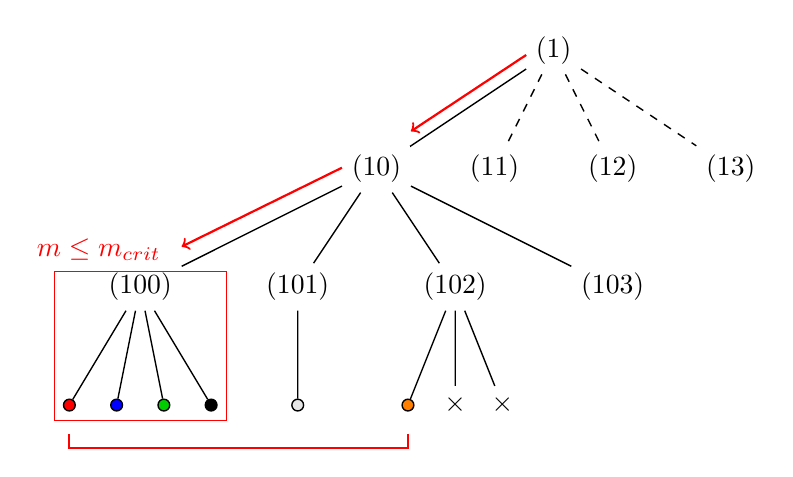
\begin{tikzpicture}

\def\da{2cm}
\def\db{20mm}
\def\dc{6mm}

\node [fill=white] at (9,0) (root) {(1)}
    child [line width=.5pt] { [sibling distance=\db] node [fill=white] (n10) {(10)}
      child {node (n100) {(100)} [sibling distance=\dc]
      	child { node[fill=red,circle,inner sep=1.5pt,draw] (n1000) {} }
      	child { node[fill=blue,circle,inner sep=1.5pt,draw] (n1001) {} }
      	child { node[fill=black!20!green,circle,inner sep=1.5pt,draw] (n1002) {} }
      	child { node[fill=black,circle,inner sep=1.5pt,draw] (n1003) {} }
      }
      child {node {(101)} [sibling distance=\dc]
      	child { node[fill=black!10,circle,inner sep=1.5pt,draw] (n1010) {} }
      }
      child {node {(102)} [sibling distance=\dc]
      	child { node[fill=orange,circle,inner sep=1.5pt,draw] (n1020) {} }
      	child { node[] (n1021) {$\times$} }
      	child { node[] (n1022) {$\times$} }
      }
      child {node {(103)} [sibling distance=\dc]
      }
    }
    child [line width=.5pt,dashed] { node [fill=white] {(11)}
    }
    child [line width=.5pt,dashed] { node [fill=white] {(12)}
    }
    child [line width=.5pt,dashed] { node [fill=white] {(13)}
    }
;
%\draw[dashed,<->,red] ([yshift=-4pt]n1000.south east) to [out=-30,in=210] ([yshift=-4pt]n1001.south west);
%\draw[dashed,<->,red] ([yshift=-4pt]n1000.south east) to [out=-30,in=210] ([yshift=-4pt]n1002.south west);
%\draw[dashed,<->,red] ([yshift=-4pt]n1000.south east) to [out=-30,in=210] ([yshift=-4pt]n1003.south west);
\draw[red,->,thick] ([yshift=7pt]root.south west) -- ([yshift=5pt]n10.north east);
\draw[red,->,thick] ([yshift=9pt]n10.south west) -- ([yshift=6pt]n100.north east);
\draw[red] ([xshift=-16pt,yshift=-3pt]n100.north west) rectangle ([xshift=4pt,yshift=-4pt]n1003.south east);
\node[red] at ([yshift=5pt]n100.north west) {$m \leq m_{crit}$};

\draw[red,thick] ([yshift=-8pt]n1000.south) |- ([yshift=-13pt]n1000.south) -- ([yshift=-13pt]n1020.south) -| ([yshift=-8pt]n1020.south);

\end{tikzpicture}
}
\caption{Neighbors search using a tree traversal per particle vs a group of particle and computing an interaction list}
\label{fig:arbre}
\end{figure}

Our search algorithm, presented on Algorithm~\ref{alg:find_nodes}, is a two-step algorithm like in Barnes trees: First create the interaction lists and then using them on the sub-tree particles. 
In the first step we look down for nodes with a target sub-mass of particles $tmass$. 
Then for those branches we compute an interaction list and continue the recursive tree search. 
When a particle is reached, we compute the physics using the interaction list as the neighbors. 
The interaction list is computing using an opening-angle criterion comparing the boundary box and a user define angle. 
This way we will not need a full tree traversal for each particle but a full tree traversal for every group of particles.
On figure~\ref{fig:arbre} we present the classical and the two steps algorithm. 
We see that the first method, on left, force to do one walk per particle, compute the interaction list and then apply to particles. 
On the left, the two-step method, only perform one tree traversal for the whole block of particles, compute the interaction list and then processed to the local computation. 
Indeed, this implies a check of particle distance during the computation since all the particles from the interaction list are not useful for every particle. 

\begin{algorithm}
\caption{Tree search algorithm}\label{alg:find_nodes}
\begin{algorithmic}[1]
\Procedure{find\_nodes}{}
\State stack $stk \leftarrow$ root
\While{not\_empty($stk$)} 
	\State branch $b \leftarrow$ $stk$.pop() 
	\If{$b$ is leaf} 
		\For{\textbf{each} particles $p$ of $b$}
			\State $apply\_sub\_tree$($p$,$interaction\_list$($p$))
		\EndFor
	\Else
		\For{\textbf{each} child branch $c$ of $b$}
			\State $stk$.push($c$)
		\EndFor
	\EndIf
\EndWhile
\EndProcedure
\State
\Procedure{apply\_sub\_tree}{node $n$, node-list $nl$}
\State stack $stk \leftarrow$ $n$
\While{not\_empty($stk$)} 
	\State branch $b \leftarrow$ $stk$.pop() 
	\If{$b$ is leaf} 
		\For{\textbf{each} particles $p$ of $b$}
			\State $apply\_physics$($p$,$nl$)
		\EndFor
	\Else
		\For{\textbf{each} child branch $c$ of $b$}
			\State $stk$.push($c$)
		\EndFor
	\EndIf
\EndWhile
\EndProcedure
\State
\Function{interaction\_list}{node $n$}
\State stack $stk \leftarrow$ root
\State node-list $nl$ $\leftarrow$ $\emptyset$
\While{not\_empty($stk$)} 
	\State branch $b \leftarrow$ $stk$.pop() 
	\If{$b$ is leaf} 
		\For{\textbf{each} particles $p$ of $b$}
			\If{within()}
				\State $nl$ $\leftarrow$ $nl$ + $p$
			\EndIf
		\EndFor
	\Else
		\For{\textbf{each} child branch $c$ of $b$}
			\If{$mac$($c$,$angle$)}
				\State $nl$ $\leftarrow$ $nl$ + $c$
			\Else				
				\State $stk$.push($c$)
			\EndIf	
		\EndFor
	\EndIf
\EndWhile
\EndFunction
\end{algorithmic}
\end{algorithm}

\subsection{Distribution strategies}

The previous section presented the tree data structure that can be use locally on every node. 
The distribution layer is added on top of it, keeping each sub-tree on the computation nodes. 
The current version of FleCSPH is still based on synchronous communications using the Message Passing Interface (MPI). 

\begin{algorithm}
\caption{Main algorithm}\label{alg:main_distributed}
\begin{algorithmic}[1]
\Procedure{specialization\_driver}{input data file $f$}
\State Read $f$ in parallel 
\State Set physics constant from $f$
\While{iterations}
\State Distribute the particles using distributed quick sort\label{alg_main:qsort}
\State Compute total range 
\State Generate the local tree
\State Share branches\label{alg_main:share_branches}
\State Compute the ghosts particles\label{alg_main:cp_ghosts}
\State Update ghosts data\label{alg_main:up_ghosts}
\State \textit{PHYSICS}
\State Update ghosts data
\State \textit{PHYSICS}
\State Distributed output to file 
\EndWhile
\EndProcedure
\end{algorithmic}
\end{algorithm}


The main distributed algorithm is presented on algorithm \ref{alg:main_distributed}:

\subsubsection{Particle distribution}

\begin{figure*}
\centering
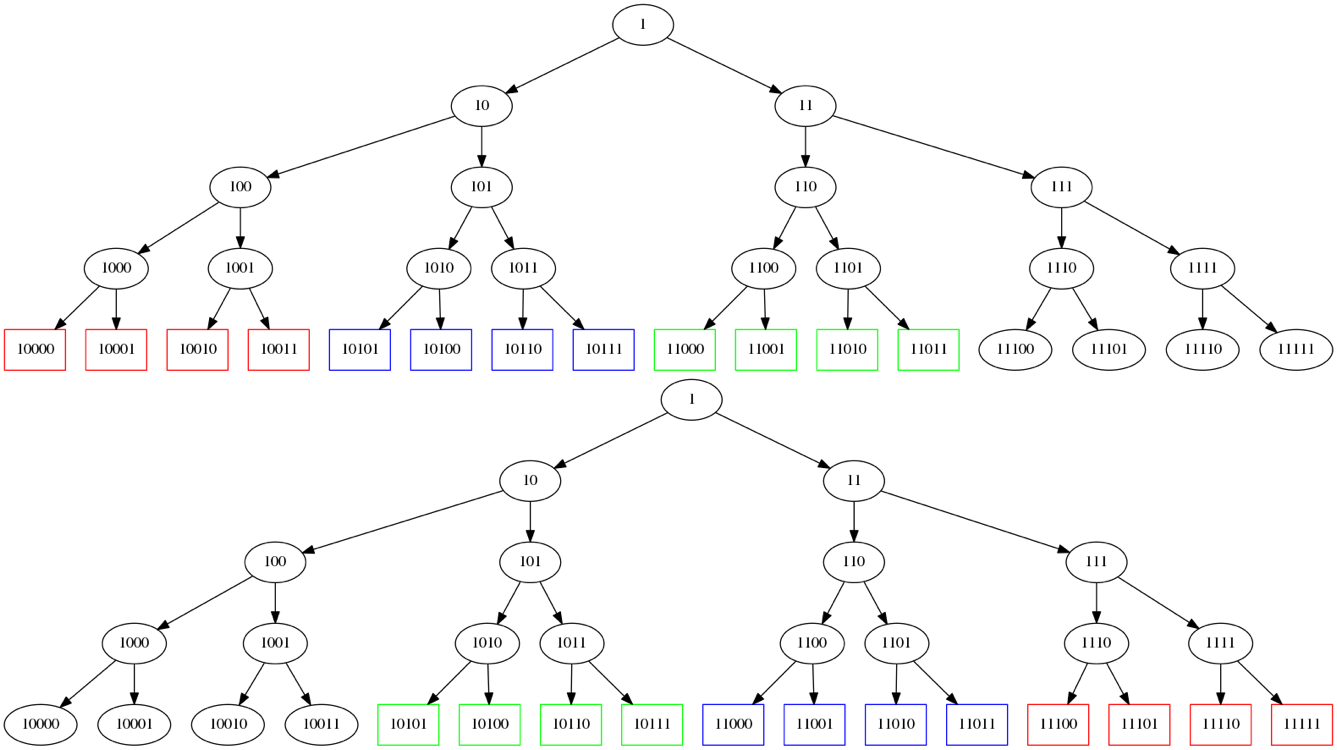
\includegraphics[width=\textwidth]{\locpath/figures/flecsph/algo.png}
\caption{Binaries tree for a 2 processes system. Exclusive, Shared and Ghosts particles resp. red, blue, green.}
\label{fig:big_tree}
\end{figure*}

The sort step, line \ref{alg_main:qsort}, is based on a distributed quick sort algorithm. 
The keys are generated using the Morton order described in part \ref{sec:domain_decomposition}. 
As we associate a unique number to each particle we are able to sort them using the keys and, in case of collision keys, using their unique ID. 
This gives us a global order for the particles. 
Each process sends to a master node (or submaster for larger cases) a sample of its keys. 
We determined this size to be 256 KB of key data per process for our test cases, but it can be refined for larger simulations. 
Then the master determines the general ordering for all the processes and shares the pivots. 
Then each process locally sorts its local keys, and, in a global communication step, the particles are distributed to the process on which they belong. 
This algorithm gives us a good partition in term of number of particles. 
But some downside can be identified:
\begin{itemize}
	\item The ordering may not be balanced in term of number of particles per processes. But by optimizing the number of data exchanged to the master can lead to better affectation. 
	\item The load balance also depend on the number of neighbors of each particle. If a particle gets affected a poor area with large space between the particles, this can lead to bad load balancing too. 
\end{itemize}
This is why we also provide another load balancing based on the particles neighbors. 
Depending on the user problem, the choice can be to distribute the particles on each process regarding the number of neighbors, having the same amount of physical computation to perform on each process. 

\begin{figure}[t!]
\centering
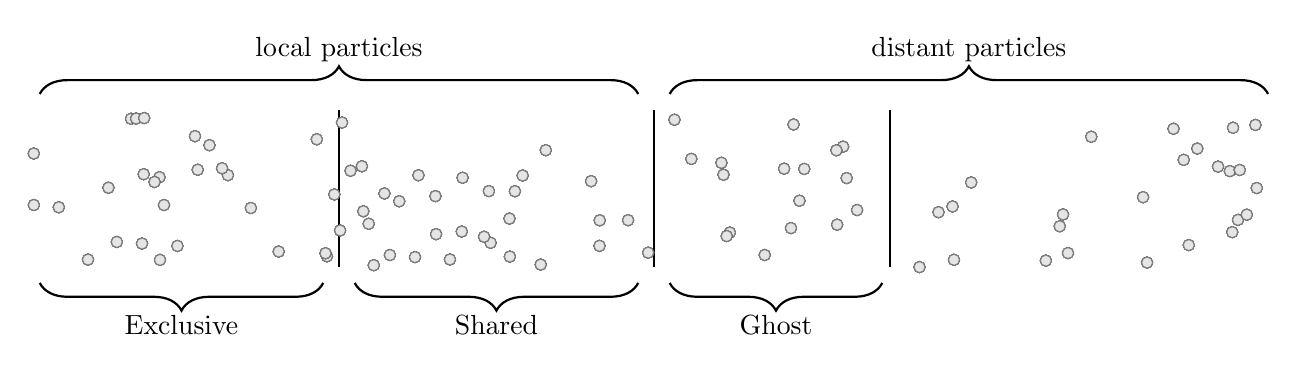
\begin{tikzpicture}
\pgfmathsetseed{1}
\def\nrand{100}
% braces on top : local; distant
\draw [thick,decorate,decoration={brace,amplitude=10pt}]
(0.2,2.2) -- (7.8,2.2) node [midway,above,yshift=8pt] 
{local particles};
\draw [thick,decorate,decoration={brace,amplitude=10pt}]
(8.2,2.2) -- (15.8,2.2) node [midway,above,yshift=8pt] 
{distant particles};

\draw [thick,decorate,decoration={brace,amplitude=10pt}]
 (3.8,-.2) -- (0.2,-.2) node [midway,below,yshift=-8pt] 
{Exclusive};
\draw [thick,decorate,decoration={brace,amplitude=10pt}]
(7.8,-.2) -- (4.2,-.2) node [midway,below,yshift=-8pt] 
{Shared};
\draw [thick,decorate,decoration={brace,amplitude=10pt}]
(10.9,-.2) -- (8.2,-.2) node [midway,below,yshift=-8pt] 
{Ghost};

% Vertical bars 
\draw[thick] (4,0) -- (4,2) node (exclusive) {};
\draw[thick] (8,0) -- (8,2) node (shared) {};
\draw[thick] (11,0) -- (11,2) node (ghosts) {};

\foreach \i in {1,2,...,\nrand}{
	\pgfmathsetmacro{\x}{((rand)+1)*8}
	\pgfmathsetmacro{\y}{((rand)+1)*1}
	\ifthenelse{ \lengthtest{\x cm < 4 cm}}
		{\draw[black!70,fill=red!90] (\x,\y) circle (2pt);}
		{\ifthenelse { \lengthtest{\x cm < 8 cm}}
			{\draw[black!70,fill=blue!90] (\x,\y) circle (2pt);}
			{\ifthenelse { \lengthtest{ \x cm < 11 cm }}
				{\draw[black!70,fill=black!30!green] (\x,\y) circle (2pt);}
				{\draw[black!50,fill=black!10] (\x,\y) circle (2pt);} 
			}
		}
}
\end{tikzpicture}
\caption{Particles "coloring" with local particles: exclusive, shared and distant particles useful during run: ghost particles}
\label{fig:coloring_particles}
\end{figure}

After this first step, the branches are shared between the different processes, line \ref{alg_main:share_branches}. 
Every of them send to its neighbors several boundaries boxes, defined by the user. 
Then particles from the neighbors are computed, exchanged and added in the local tree. 
Those particles are labeled as NON\_LOCAL particles. 
At this point a particle can be referenced as: EXCLUSIVE: will never be exchanged and will only be used on this process; SHARED: may be needed by another process during the computation; GHOSTS: particles information that the process need to retrieve from another process. 
An example is given for 2 processes on figure~\ref{fig:coloring_particles} and on a tree data structure on figure~\ref{fig:big_tree}.

\subsubsection{Exchange Shared and Ghosts particles}

The previous distribution shares the particles and the general information about neighbors particles. 
Then each process is able to do synchronously or asynchronously communications to gather distant particles. 
In the current version of FleCSPH an extra step is required to synchronously share data of the particles needed during the next tree traversal and physics part. 
Then after this step, the ghosts data can be exchanged as wanted several times during the same time step. 

\subsection{Fast Multipole Methods}

We described in the previous chapter a method to compute gravitational interactions faster than the $O(N^2)$ n-body algorithm, the Fast Multipole Method, FMM.
This allows an approach with a precision depending of a parameter called the Multipole Acceptance Criterion, MAC. 
This is needed for us to target binary neutron stars simulations with high number of particles.

This approach is also based on the tree topology used for the SPH method. 
Three main functions are used: 
\begin{itemize}
	\item \begin{verbatim}mpi_exchange_cells\end{verbatim} share the centers of mass computed in the tree up to a determined mass. By default, the program shares the lowest COM, the leaves. 
	\item \begin{verbatim}mpi_compute_fmm\end{verbatim} After gathering the COM this step performs the M2M computation and also isolate the particles needed for the distant P2P step. 
	\item \begin{verbatim}mpi_gather_cells\end{verbatim} Gather The contribution of all the other processes and sum in the local branch.
	Then this step performs both the M2P and P2P computations. 
	A specific P2P for distant particles is added to take in account the particles found on other processes in the M2M step.
\end{itemize}

\begin{figure}[t!]
\centering
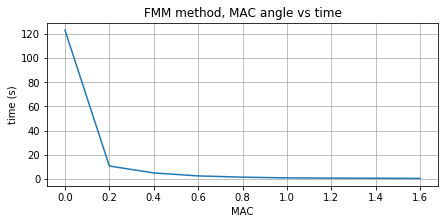
\includegraphics[width=.45\columnwidth]{\locpath/figures/flecsph/fmm_mac.png}
\caption{Evolution of time regarding the multipole acceptance criterion for FMM method.}
\label{fig:mac_angle}
\end{figure}

The speed of computation varies with the choose of the MAC angle. 
An example is given on figure~\ref{fig:mac_angle}.
It presents the time varying with the angle. 
We note that bigger the angle, faster the computation time. 
The limit of the angle is $\Theta =  \frac{\pi}{2}$.
The loss of precision can be quantified with the evolution of linear and angular momentum.
We fixed our MAC to $\Theta = 1$.

\subsection{I/O}
Regarding the high number of particles, an efficient, parallel and distributed I/O implementation is required. 
Several choices were available, but we wanted a solution that can be specific for our usage. 
The first requirement is to allow the user to work directly with the Paraview visualization tool and splash\footnote{\url{http://users.monash.edu.au/~dprice/splash/}}~\cite{price2007splash}.

We base this first implementation on HDF5~\cite{folk1999hdf5} file structure with H5Part and H5Hut~\cite{howison2010h5hut}. 
HDF5 support MPI runtime with distributed read and write in a single or multiple file. 
We added the library H5hut to add normalization in the code to represent global data, steps, steps data and the particles data for each step.
The I/O code was developed internally at LANL and provides a simple way to write and read the data in H5Part format. 
The usage of H5Hut to generate H5part data files allows us to directly read the output in Paraview without using a XDMF descriptor like requested in HDF5 format.

\section{Distributed SPH on hybrid architectures}
We constructed an efficient and reliable SPH code working on classical architecture clusters. 
In this section we present our multi-GPU implementation and compare it with our multi-CPU code. 
We kept the same data structure, distribution strategy and code architecture in the accelerator code. 
Several options are possible for the accelerator implementation, but we wanted to keep the code usable and working for the domain scientists. 
As the current version of FleCSI does not allow utilization of accelerator like GPU for the data structure, we decided to embed the GPU code directly on FleCSPH. 
We provided the same approach we studied in the Langford problem offloading part of the tree computation on the accelerators. 

\subsection{Distribution strategies} 
The FleCSPH framework provides all the tools and distribution strategies for multi-CPU and distributed computation.
In order to target hybrid architectures several approaches were possible.
They were identified in the previous metrics for the Langford problem.
The first one is to implement the whole tree traversal and data representation on GPU. 
This strategy imposes several downsides especially for asynchronous communication.
The data structure of FleCSI and FleCSPH does not allows the full transformation of the data structure into CUDA code and, furthermore, this would transform the framework into a problem dependent API. 
Even if the performances would be slightly better, the aim of this framework is to target multi-physics problems and thus general.

The second strategy is the one used in the Langford problem case. 
The smoothing length computation is a tree traversal that's lead to a group of particles and their neighbors. 
We decided to offload the physics computation on accelerators. 

\begin{figure}[t!]
\resizebox {\columnwidth} {!} {
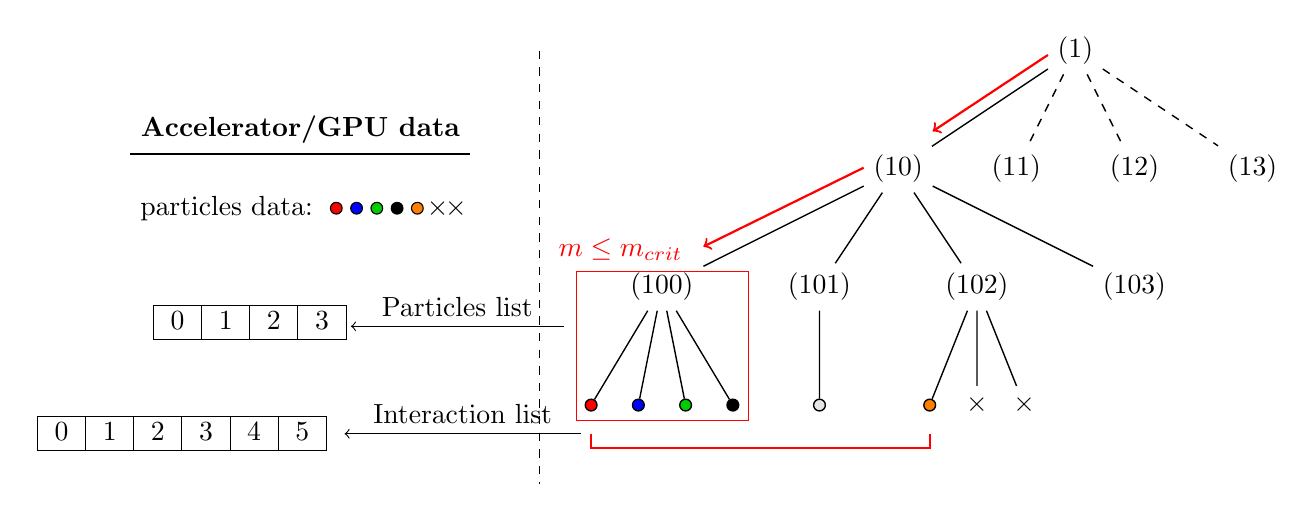
\begin{tikzpicture}

\def\da{2cm}
\def\db{20mm}
\def\dc{6mm}

\node [fill=white] at (9,0) (root) {(1)}
    child [line width=.5pt] { [sibling distance=\db] node [fill=white] (n10) {(10)}
      child {node (n100) {(100)} [sibling distance=\dc]
      	child { node[fill=red,circle,inner sep=1.5pt,draw] (n1000) {} }
      	child { node[fill=blue,circle,inner sep=1.5pt,draw] (n1001) {} }
      	child { node[fill=black!20!green,circle,inner sep=1.5pt,draw] (n1002) {} }
      	child { node[fill=black,circle,inner sep=1.5pt,draw] (n1003) {} }
      }
      child {node {(101)} [sibling distance=\dc]
      	child { node[fill=black!10,circle,inner sep=1.5pt,draw] (n1010) {} }
      }
      child {node {(102)} [sibling distance=\dc]
      	child { node[fill=orange,circle,inner sep=1.5pt,draw] (n1020) {} }
      	child { node[] (n1021) {$\times$} }
      	child { node[] (n1022) {$\times$} }
      }
      child {node {(103)} [sibling distance=\dc]
      }
    }
    child [line width=.5pt,dashed] { node [fill=white] {(11)}
    }
    child [line width=.5pt,dashed] { node [fill=white] {(12)}
    }
    child [line width=.5pt,dashed] { node [fill=white] {(13)}
    }
;
\draw[red,->,thick] ([yshift=7pt]root.south west) -- ([yshift=5pt]n10.north east);
\draw[red,->,thick] ([yshift=9pt]n10.south west) -- ([yshift=6pt]n100.north east);
\draw[red] ([xshift=-16pt,yshift=-3pt]n100.north west) rectangle ([xshift=4pt,yshift=-4pt]n1003.south east) node[anchor=west] (leaf) {};
\node[red] at ([yshift=5pt]n100.north west) {$m \leq m_{crit}$};

\draw[red,thick] ([yshift=-8pt]n1000.south) node (list_inter) {} |- ([yshift=-13pt]n1000.south) -- ([yshift=-13pt]n1020.south) -| ([yshift=-8pt]n1020.south);

% GPU Computation
\node[anchor=west,thick,font=\bf] at (-3,-1) (accel) {Accelerator/GPU data};
\draw[thick] (accel.south west) -- (accel.south east);

\node[anchor=west] at (-3,-2) (pd) {particles data:};
\node[fill=red,circle,inner sep=1.5pt,draw] at ([xshift=5pt]pd.east) (a) {};
\node[fill=blue,circle,inner sep=1.5pt,draw] at ([xshift=5pt]a.east) (b) {};
\node[fill=black!20!green,circle,inner sep=1.5pt,draw] at ([xshift=5pt]b.east) (c) {};
\node[fill=black,circle,inner sep=1.5pt,draw] at ([xshift=5pt]c.east) (d) {};
\node[fill=orange,circle,inner sep=1.5pt,draw] at ([xshift=5pt]d.east) (e) {};
\node[inner sep=1.5pt] at ([xshift=5pt]e.east) (f) {$\times$};
\node[inner sep=1.5pt] at ([xshift=1pt]f.east) (g) {$\times$};

\draw[->] (2.5,-3.5) -- ([xshift=-2.7cm]2.5,-3.5) node[midway,above] (leaf_node) {Particles list};
\node[anchor=east] at ([xshift=-.2cm,yshift=-.2cm]leaf_node.west) { 
	\begin{tabular}{|c|c|c|c|}
		\hline
		0 & 1 & 2& 3\\
		\hline
  	\end{tabular}	
};
\draw[->] (list_inter.west) -- ([xshift=-3cm]list_inter.west) node[midway,above] (inter) {Interaction list};
\node[anchor=east] at ([xshift=-3.1cm]list_inter.west) { 
	\begin{tabular}{|c|c|c|c|c|c|}
		\hline
		0 & 1 & 2 & 3 & 4 & 5\\
		\hline
  	\end{tabular}	
};

\draw[dashed] (2.2,0) -- (2.2,-5.5);


\end{tikzpicture}
}
\caption{Task resolution using GPUs}
\label{fig:multi_gpu_implementation}
\end{figure}
Figure~\ref{fig:multi_gpu_implementation} presents the distribution of tasks with the accelerator. 
The tree traversal itself stays on the host processor and lower part of the tree are offloaded to the accelerators. 
The traversal is done in parallel on the host and, when a group of particles and its neighbors list is reached, the data are transferred to the GPU for computation. 
With this method the GPU is fully used for regularized computation and the CPU handle the data structure. 
When the tree traversal is done, the CPU wait for last GPU tasks to complete and can gather the result or start another traversal leaving data on GPUs. 

\subsection{Physics on accelerators}
The computation of physics is also slightly different on accelerators. 
Indeed, the CPU send to the GPU indexes with the particles and their possible neighbors. 
The GPU perform a brute force computation with $O(n^2)$ algorithm. 
It keeps checking if the particles received are inside the smoothing length radius. 
The target particle is loaded in local memory and its neighbors are stored in the local memory for a WARP based computation.
The threads then iterate on the local particles and output together in global memory.

\section{Results}
In this part we compare the results of the multi-GPU version and the multi-CPU version of FleCSPH. 
We show the benefit of using hybrid architecture even on irregular problem with high communications and computations.

\subsection{Performances}
The two metrics we worked on, in part II, gave us hint in order to reach performances in this simulation code. 
The first step was to find the best repartition between the host and device.

\begin{figure}[t!]
\centering
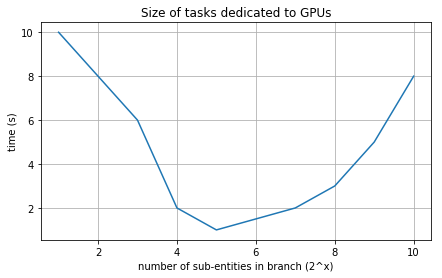
\includegraphics[width=.45\textwidth]{\locpath/figures/flecsph/task_gpu.png}
\caption{CPU-GPU tasks work balancing}
\label{fig:cpu_gpu_rep}
\end{figure}%

Figure~\ref{fig:cpu_gpu_rep} shows the work balancing. 
With the smallest distribution the CPU and GPU keep exchange data for very small amount of computation. 
Art the opposite, if the CPU value is too high the $O(n^2)$ part is too important. 
We choose the value to be configured by the user and defaulted at  XX.

\begin{figure}[t!]
\centering
\begin{minipage}[b]{.45\textwidth}
\centering
	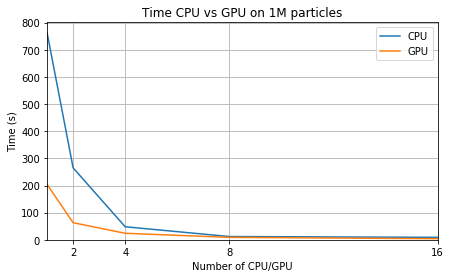
\includegraphics[width=\textwidth]{\locpath/figures/flecsph/time_CPU_vs_GPU.png}
	\caption{CPU vs GPU time per iteration}
	\label{fig:cpu_gpu_time}
\end{minipage}
\begin{minipage}[b]{.45\textwidth}
\centering
	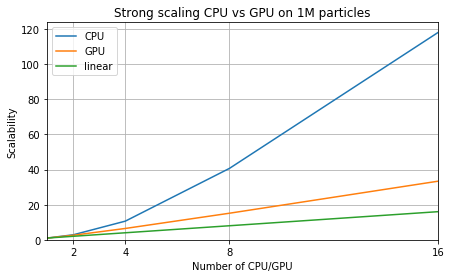
\includegraphics[width=\textwidth]{\locpath/figures/flecsph/scalability_CPU_vs_GPU.png}
	\caption{CPU vs GPU scalability per iteration}
	\label{fig:cpu_gpu_scala}
\end{minipage}
\end{figure}

On figure~\ref{fig:cpu_gpu_time} and figure~\ref{fig:cpu_gpu_scala} we find the strong scaling and scalability tests for CPU and GPU version using the empiric best depth of repartition.
The time comparison with strong scaling shows us that the GPU version go faster than the CPU one with a peak of 5 times faster. 
On the other hand, the scalability graph present that the CPU version is more scalable than the GPU version. 
This can be explain in two ways.

\subsection{Simulations}
The results and tests were done on several physical and astrophysical simulations in order to check the code behavior and reliability. 
\begin{figure}[t!]
\centering
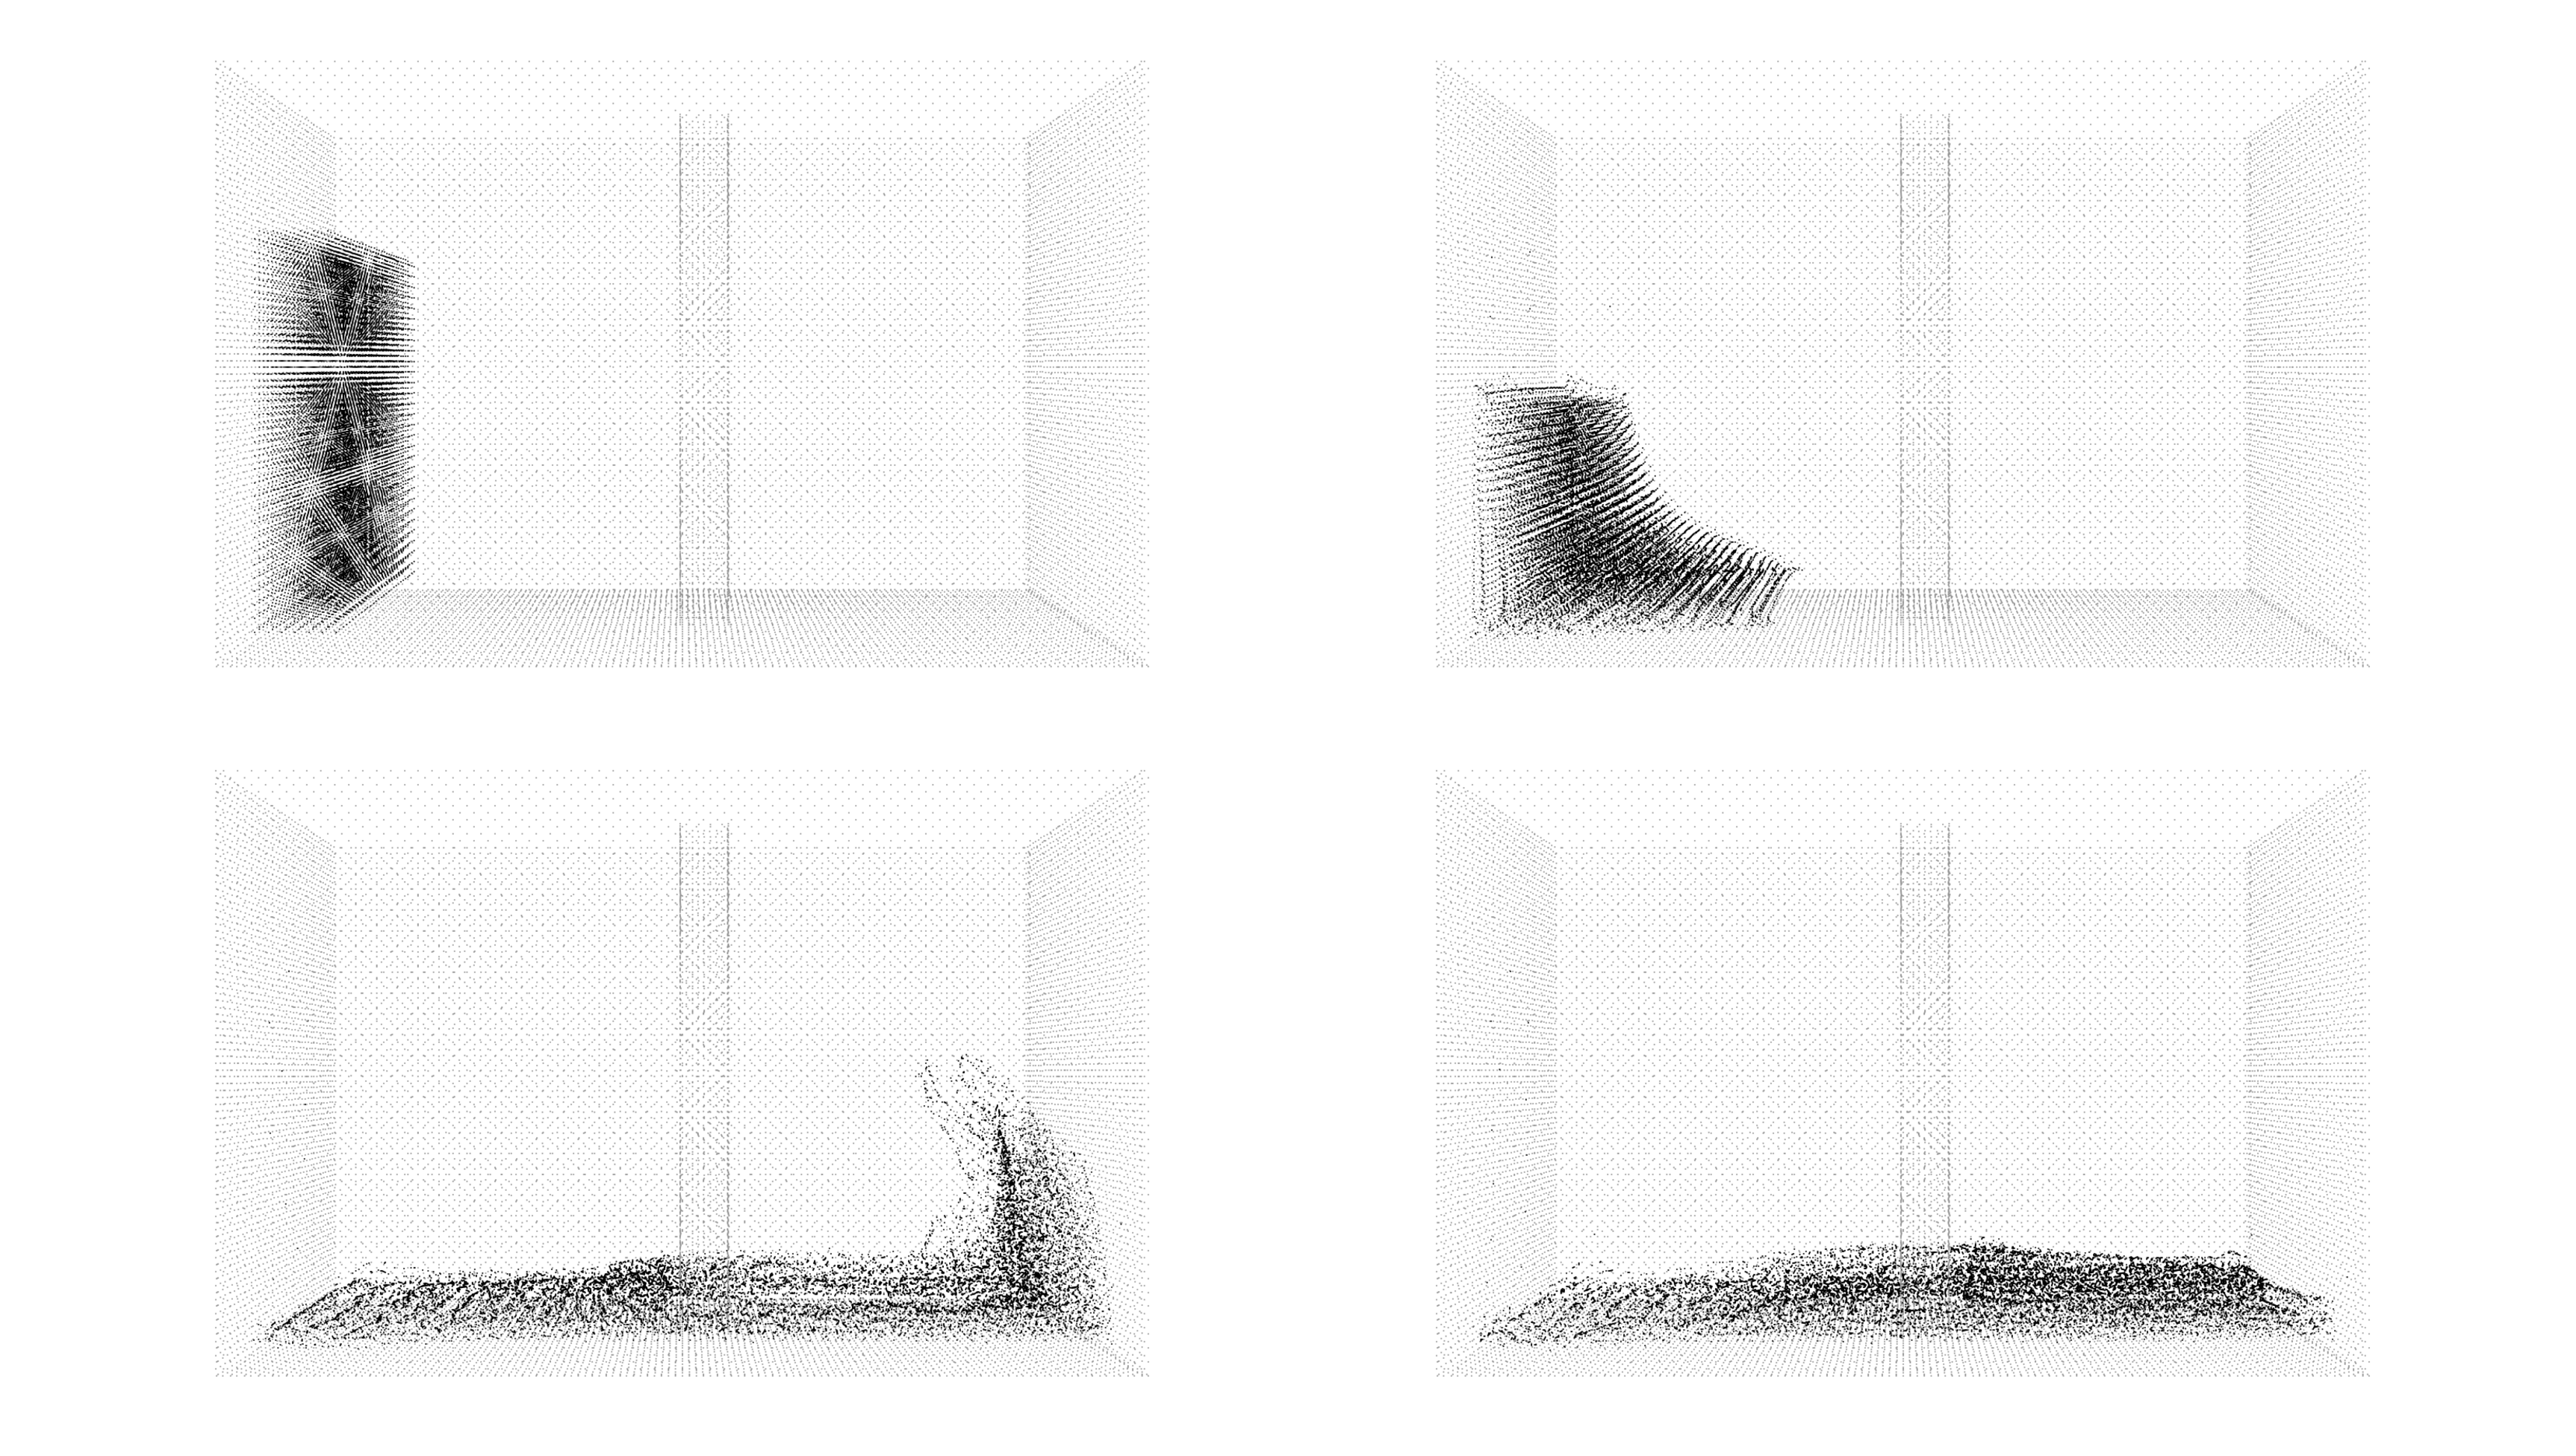
\includegraphics[width=\textwidth]{\locpath/figures/sph/fluid_flow}
\caption{Fluid flow simulation, the dam break. For $t=0$, $t=0.4$, $t=0.8$ and $t=1$ seconds}
\label{fig:fluid_simulation}
\end{figure}

The first tests, done on Sod shock tube and Sedov blast wave were presented in the previous chapter, showed perfect results. 

The fluid simulation is presented on figure~\ref{fig:fluid_simulation}.
In this figure we can see a 40,000 particles simulation executed on multiples node of the ROMEO supercomputer. 
This dam break simulation gave us the opportunity to represent the behavior of boundary conditions with a high number of particles. 

In order to target a problem with both SPH and gravitation we decided to work on Astrophysics events like Binary Neutron Stars.
The initial data were generated using python 3.5 to compute the position, mass and smoothing length of every particles. 
A first step is done for the relaxation, the particles take their location. 
The system relaxed then evolve following the merging equations proposed in the previous chapter. 
\begin{figure}[t!]
\centering
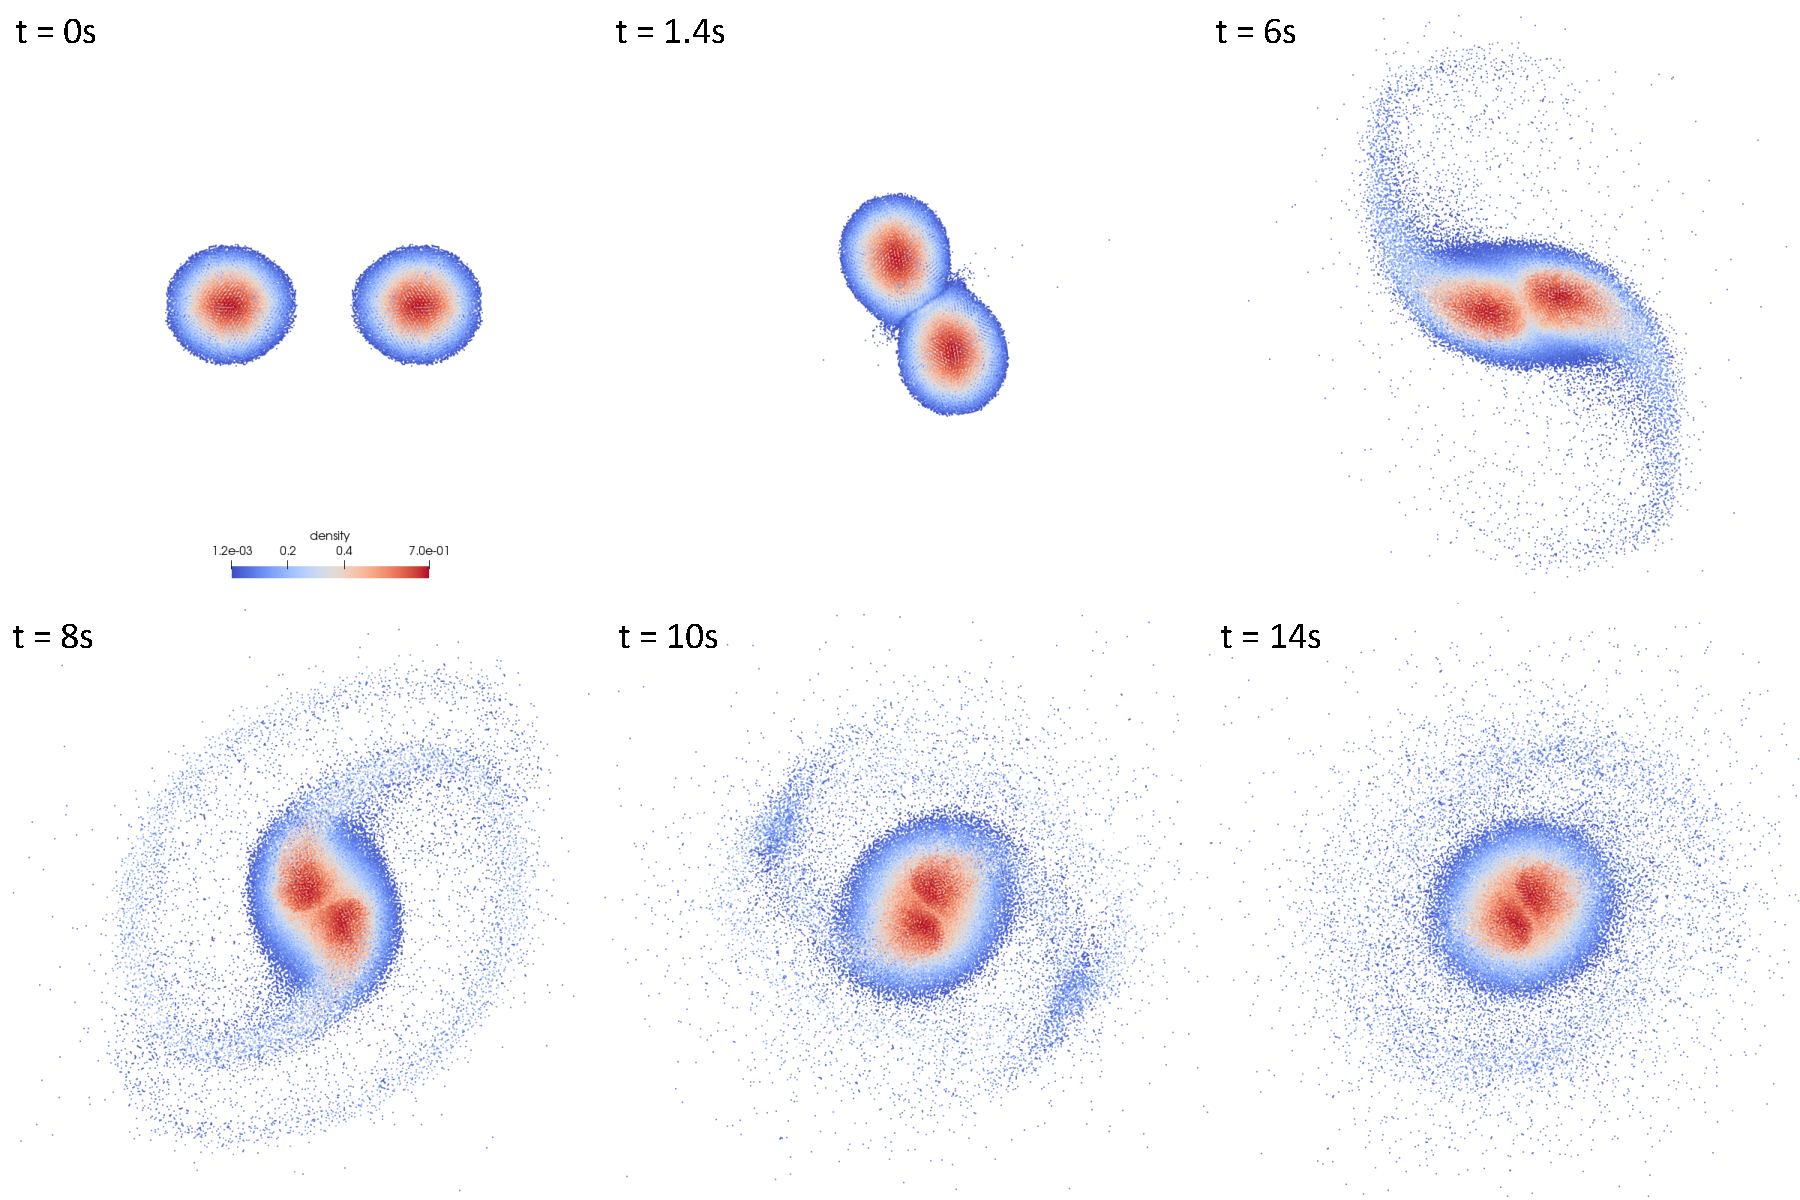
\includegraphics[width=\textwidth]{\locpath/figures/flecsph/bns_merger}
\caption{Binary Neutron Stars coalescence with 40.000 particles.}
\label{fig:bns_simulation}
\end{figure}

Figure~\ref{fig:bns_simulation} presents the binary neutron star coalescence for 40,000 particles. 
The computation took 5 hours on four nodes of the supercomputer ROMEO. 
This simulation is done with a total of 750 outputted steps with more than 100,000 iterations. 

\section{Conclusion}
In this section we presented a tool completing our metric. 
This production application dedicated to smoothed particles hydrodynamics and gravitation simulation is called FleCSPH. 
It allows us to target both computation and communication walls in a highly irregular context.

We based our hybrid implementation on the knowledge from the two first metric of our benchmark.
We showed the advantage of using hybrid architecture on this kind of application and this behavior can be find in many others. 

It is important to notice that the GPU usage is not the best in this case. 
Indeed, a dedicated application for each specific SPH problem would be more efficient. 
The aim is to provide a framework that can be use on a large set of cluster and architectures. 
Even with those limitations, the GPU was able to provide an acceleration of up to 5 times faster compare to the full-CPU computation. 